\noindent 
In this project, we envision to develop a PIM system depicted in Figure~\ref{fig:arch}. 
Overall, the system consists of an accelerator-memory (AM) HIVE and conventional host systems. 
An AM HIVE is comprised of multiple nodes (or packages) connected by our power-efficient high-bandwidth chip-to-chip links in a mesh style. 
One accelerator (ACC) and four 8GB DiRAM4 dies will constitute a PIM package with 4TB/s aggregate in-package bandwidth. 
Our ACC die will integrate 32 ACCs with our custom eDRAM, a 32×32 crossbar, and a network interface (NI) to support chip-to-chip communications.

\begin{wrapfigure}{r}[0pt]{0.7\textwidth}
\center
%\vspace{-8ex}
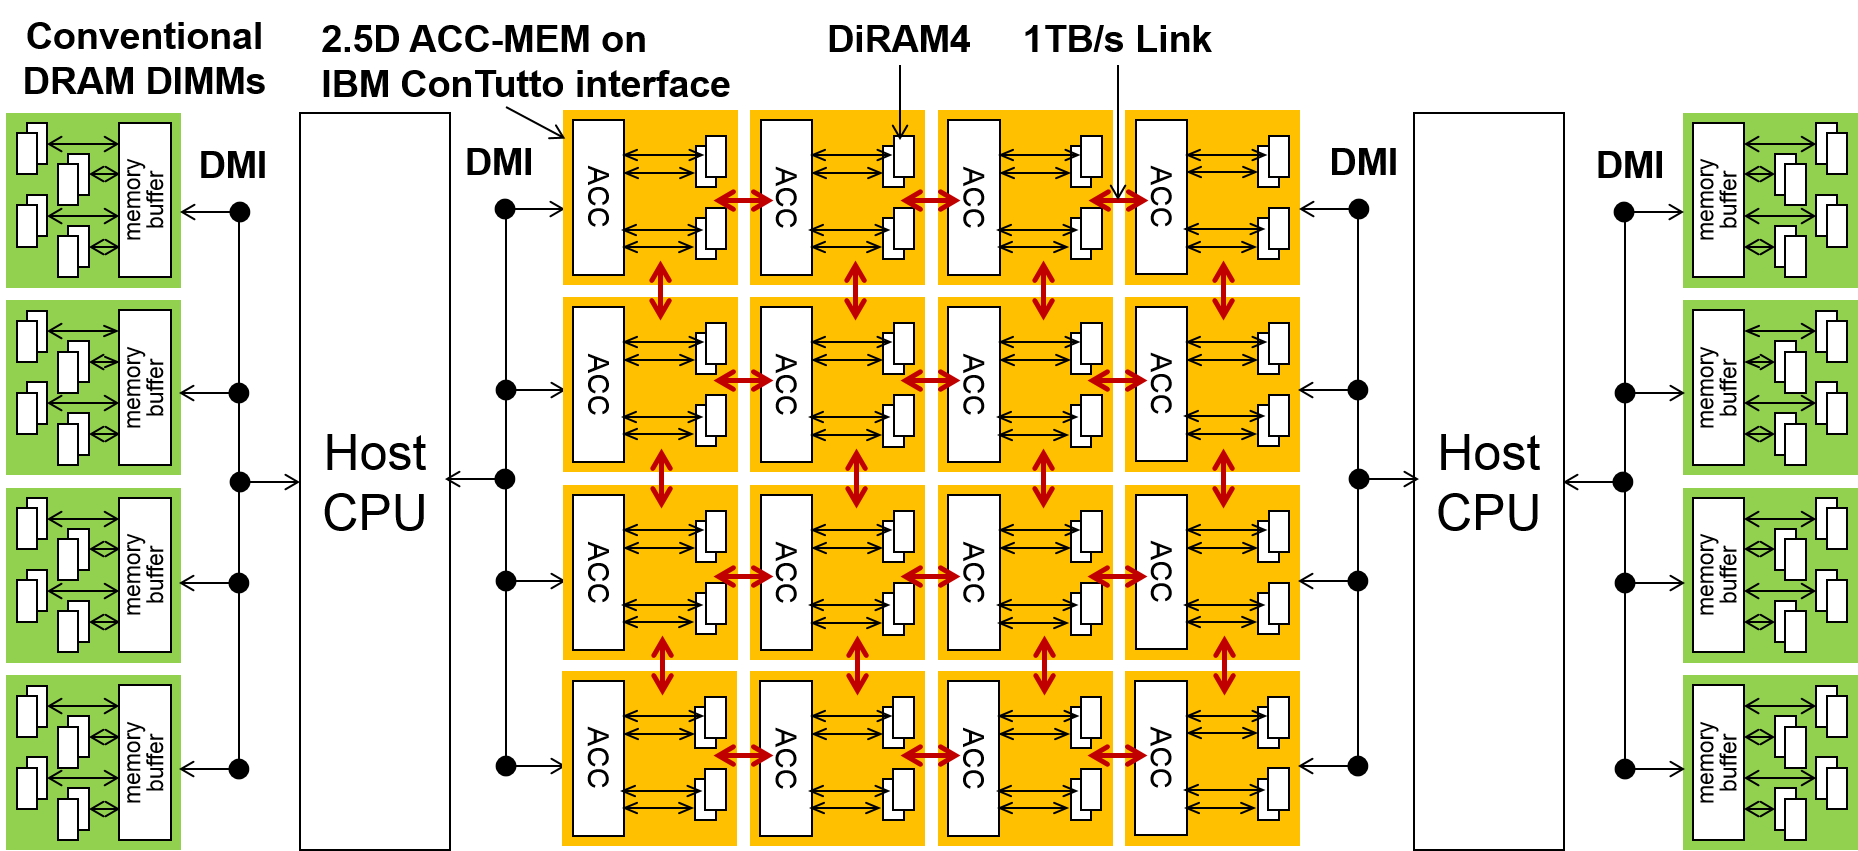
\includegraphics[width=1.0\linewidth]{./fig/arch.png}
\caption{The overall architecture of an Accelerator-Memory HIVE.}
\label{fig:arch}
\end{wrapfigure}
